\documentclass[border=5pt]{standalone}
\usepackage{tikz}
\usetikzlibrary{calc, positioning}
\usepackage{amsmath}
\begin{document}
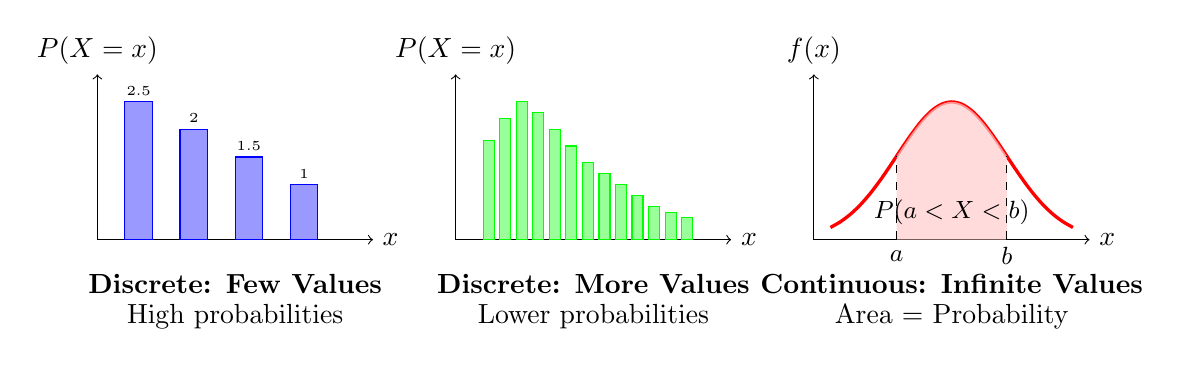
\begin{tikzpicture}[scale=0.7]
% Discrete distribution with few values
\begin{scope}[xshift=0cm]
\draw[->] (0,0) -- (5,0) node[right] {$x$};
\draw[->] (0,0) -- (0,3) node[above] {$P(X = x)$};
\draw[fill=blue!40, draw=blue] (0.5,0) rectangle (1,2.5);
\draw[fill=blue!40, draw=blue] (1.5,0) rectangle (2,2);
\draw[fill=blue!40, draw=blue] (2.5,0) rectangle (3,1.5);
\draw[fill=blue!40, draw=blue] (3.5,0) rectangle (4,1);
\node at (2.5,-0.8) {\textbf{Discrete: Few Values}};
\node at (2.5,-1.4) {High probabilities};
\foreach \x/\y in {0.75/2.5, 1.75/2, 2.75/1.5, 3.75/1}
  \node at (\x,\y+0.2) {\tiny \y};
\end{scope}

% Discrete distribution with more values
\begin{scope}[xshift=6.5cm]
\draw[->] (0,0) -- (5,0) node[right] {$x$};
\draw[->] (0,0) -- (0,3) node[above] {$P(X = x)$};
\foreach \x/\h in {0.5/1.8, 0.8/2.2, 1.1/2.5, 1.4/2.3, 1.7/2.0, 2.0/1.7, 2.3/1.4, 2.6/1.2, 2.9/1.0, 3.2/0.8, 3.5/0.6, 3.8/0.5, 4.1/0.4} {
  \draw[fill=green!40, draw=green] (\x,0) rectangle (\x+0.2,\h);
}
\node at (2.5,-0.8) {\textbf{Discrete: More Values}};
\node at (2.5,-1.4) {Lower probabilities};
\end{scope}

% Continuous distribution
\begin{scope}[xshift=13cm]
\draw[->] (0,0) -- (5,0) node[right] {$x$};
\draw[->] (0,0) -- (0,3) node[above] {$f(x)$};
\draw[red, very thick] plot[smooth, domain=0.3:4.7] (\x, {2.5*exp(-(\x-2.5)^2/2)});
\fill[red!20, opacity=0.7] plot[smooth, domain=1.5:3.5] (\x, {2.5*exp(-(\x-2.5)^2/2)}) -- (3.5,0) -- (1.5,0) -- cycle;
\draw[dashed] (1.5,0) -- (1.5,{2.5*exp(-(1.5-2.5)^2/2)});
\draw[dashed] (3.5,0) -- (3.5,{2.5*exp(-(3.5-2.5)^2/2)});
\node at (2.5,-0.8) {\textbf{Continuous: Infinite Values}};
\node at (2.5,-1.4) {Area = Probability};
\node at (2.5,0.5) {\small $P(a < X < b)$};
\node at (1.5,-0.3) {\small $a$};
\node at (3.5,-0.3) {\small $b$};
\end{scope}
\end{tikzpicture}
\end{document}
